\documentclass[a4paper, twoside, 11pt]{report}

\usepackage[utf8]{inputenc}
\usepackage[T1]{fontenc}
\usepackage[english]{babel}
\usepackage[top= 120pt, left=80pt, right=80pt]{geometry} %marges
\usepackage{setspace} %interlignage
\usepackage{url}
\usepackage{graphicx}
\usepackage{lmodern}
\usepackage{array}
\usepackage{csquotes}
\usepackage[numbers,square]{natbib}
\usepackage{soul}
\usepackage{hyperref}
\usepackage{amsthm}
\usepackage{color}
\usepackage[usenames,dvipsnames,svgnames,table]{xcolor}
\usepackage{adjustbox}
\usepackage{amssymb}
\usepackage{amsmath}
\usepackage{dsfont}
\usepackage{physics}
\usepackage{amsfonts}
\usepackage[numbers,square]{natbib}
\usepackage{multirow}
\usepackage{listings}
\usepackage{wasysym}
\usepackage{algpseudocode}
\usepackage[ruled]{algorithm2e}
\usepackage{caption}


%%%%%% COULEURS CODE C++
\lstdefinestyle{customc}{
  belowcaptionskip=1\baselineskip,
  breaklines=true,
  frame=L,
  xleftmargin=\parindent,
  language=C,
  showstringspaces=false,
  basicstyle=\footnotesize\ttfamily,
  keywordstyle=\bfseries\color{red},
  commentstyle=\itshape\color{gray},
  identifierstyle=\color{NavyBlue},
  stringstyle=\color{black},
}

\lstdefinestyle{customasm}{
  belowcaptionskip=1\baselineskip,
  frame=L,
  xleftmargin=\parindent,
  language=[x86masm]Assembler,
  basicstyle=\footnotesize\ttfamily,
  commentstyle=\itshape\color{purple!40!black},
}

\lstset{escapechar=@,style=customc}

%%%%%% STYLES DE THÉORÈMES

\newtheoremstyle{theorem}%	Name
  {}%	Space above
  {}%	Space below
  {}%	Body font
  {}%	Indent amount
  {\bfseries}%	Theorem head font
  {.}%	Punctuation after theorem head
  { }%	Space after theorem head, ' ', or \newline
  {}%	Theorem head spec (can be left empty, meaning `normal')

\newtheoremstyle{exemple}%	Name
  {}%	Space above
  {}%	Space below
  {\color{Gray}\itshape}%	Body font
  {}%	Indent amount
  {\color{Gray}\itshape}%	Theorem head font
  {.}%	Punctuation after theorem head
  { }%	Space after theorem head, ' ', or \newline
  {}%	Theorem head spec (can be left empty, meaning `normal')

\newtheoremstyle{remark}%	Name
  {}%	Space above
  {}%	Space below
  {\itshape}%	Body font
  {}%	Indent amount
  {\bfseries}%	Theorem head font
  {.}%	Punctuation after theorem head
  { }%	Space after theorem head, ' ', or \newline
  {}%	Theorem head spec (can be left empty, meaning `normal')

%%%%%% DÉCLARATION DES THÉORÈMES

\theoremstyle{theorem}
\newtheorem{theorem}{Theorem}[section]
\newtheorem{lemme}{Lemma}[section]
\newtheorem{proposition}{Proposition}[section]
\newtheorem{definition}{Definition}[section]

\theoremstyle{remark}
\newtheorem{remark}{Remark}[chapter]

\theoremstyle{exemple}
\newtheorem*{exemple}{Example}

\newcommand{\mimi}{\mathrm{Je\ t'aime}}

\newcommand{\N}{\mathbb{N}}
\newcommand{\Z}{\mathbb{Z}}
\newcommand{\R}{\mathbb{R}}
\newcommand{\C}{\mathbb{C}}
\newcommand{\dx}{$\Delta x$ \ }

\newcolumntype{M}[1]{>{\centering\arraybackslash}m{#1}} %Pour personnaliser la largeur des colonnes dans des tabular tout en restant centré



%%%%%%%%%%%%%%%%%%%%%%%%%%%%%%%%%%%%%%%%%%%%%%%%%%%%%%%
%%%%%%%%%%%%%%%%%%%%%%%%%%%%%%%%%%%%%%%%%%%%%%%%%%%%%%%
%%%%%%%%%%%%%%%%%%%%%%%%%%%%%%%%%%%%%%%%%%%%%%%%%%%%%%%

\title{FYS3150\\Project 5}
\author{Antoine Hugounet \& Ethel Villeneuve}
\date{December 2017 \\University of Oslo \\ \url{https://github.com/kryzar/Calypso.git}}


\begin{document}
\selectlanguage{english}
\maketitle


\begin{abstract}

    This project aims to resolve numerically the diffusion equation in both one and two spatial dimensions. We implement explicit, implicit and Crank-Nicolson schemes in one dimension, implicit scheme in two dimensions, investigate their stability properties and compare them. We also study the diffusion process with videos we have made and observe the differences in the convergences to the steady state when we vary the boundary conditions. The results are convincing and reliables, yet the errors of the schemes do not behave as expected. However the schemes, except the explicit scheme in one dimension, are very close to the analytical result, with a relative error inferior to ${10}^{-3}$ if we choose our parameters wisely.

\end{abstract}


\tableofcontents


\chapter*{Introduction}
\addcontentsline{toc}{chapter}{Introduction}

    \paragraph{}This project is another project dealing with finite-difference methods. But this time we gather several methods we have studied earlier (iterative solvers, gaussian elimination) to compute PDEs. The classical formulae for the first derivative of a function (forward formula, backward formula, average of the two previous formulae) however leads to very different mathematical methods : the explicit scheme, the implicit scheme and the Crank-Nicolson scheme. \\
    However their use comes with many constraints regarding stability and mathematical errors. That's why we spend a lot of time discuting about how to choose the parameters for the solvers, how the Von Neumann stability analysis evaluates the theoritical errors and how it does not always match the informatic reality. Yet you will see plots full of colors and simulations that show very well how the diffusion of temperature occurs.


\chapter{Theory and algorithms}

    \section{One space-dimension equation}

        \paragraph{}We start with

        \begin{equation*}
                \frac{\partial^2u(x,t)}{\partial x^2}=\frac{\partial u(x,t)}{\partial t}\text{, \hspace{0.5cm}$t>0$, $x\in[0,L]$}
                \tag{1}
            \end{equation*}

            We set the initial conditions to be :

            \begin{align*}
                u(x,0)&=0\text{, \hspace{1cm} $0<x<L$}\\
                u(0,t)&=0\text{, \hspace{1cm} $t>0$}\\
                u(L,t)&=1\text{, \hspace{1cm} $t>0$}
            \end{align*}

        We scale the equations by choosing $L=1$ and we will use the more compact notation $u_{xx}=u_t$. We will consider three methods for partial differential equations : the explicit forward Euler algorithm, the implicit backward Euler algorithm and the implicit Crank-Nicolson scheme.

            \subsection{Analytical solution}

                \paragraph{}We introduce $\widetilde{u}(x,t)$ as $u(x,t)=\frac{x}{L} + \widetilde{u}(x,t)$ because the boundary conditions of $u$ ($u(0,t)=0$ and $u(L,t)=1$) do not allow us to simplify enough the equations. Considering $\widetilde{u}$, the boundary conditions are

                    \begin{equation*}
                       \widetilde{u}(0,t)=\widetilde{u}(L,t)=0
                    \end{equation*}
                %
                Then :
                    \[
                        u_t = u_{xx} \Longrightarrow \widetilde{u}_t = \widetilde{u}_{xx}
                    \]
                %
                Let's solve the equation for $\widetilde{u}$. We assume that the solution takes the form of $\widetilde{u}(x,t)=F(x).G(x)$ by separation of variables.

                    \begin{align*}
                        \left\{ \begin{matrix}
                                    \widetilde{u}_t=F\dot{G}\\
                                    \widetilde{u}_{xx}=F''G
                              \end{matrix} \right. &\Longrightarrow \frac{\dot{G}}{G}= \frac{F''}{F}=k
                        \Longrightarrow \left\{\begin{matrix}
                                                    F''-kF=0 \\
                                                    \dot{G}-kG=0
                                                \end{matrix} \right.
                    \end{align*}
                %
                We begin with the first equation $F''-kF=0$. The discriminant of this equation is $\Delta = k^2$. The only valid case $\sqrt{\Delta}=k<0$, otherwise we end up with $F=0$. In that case, we have a solution of the form : $F(x) = A \cos(\sqrt{|k|}x) + B \sin (\sqrt{|k|}x)$. Applying the boundary conditions we have $F(0)=A=0$ and $F(L)=B \sin (\sqrt{|k|}L)=0$. The latest equation implies $\sin(\sqrt{|k|}L)=0 \Longrightarrow \sqrt{|k|}L=n\pi \Longleftrightarrow \sqrt{|k|}=n \frac{\pi}{L}$ for any integer $n$. Then :

                    \begin{equation*}
                        F_n(x)=B_n \sin n\frac{\pi}{L}x
                        \tag{2}
                    \end{equation*}

                Now, we take the second equation : $\dot{G}-kG=0$. This has solutions of the form $G_n(t)=C_ne^{-\lambda^2_nt}$ with $\lambda_n=\frac{n\pi}{L}$. Then :

                    \begin{equation*}
                        \widetilde{u}(x,t)=\widetilde{u}_n(x,t)=D_n\sin(\frac{n\pi x}{L})e^{-\left(\frac{n\pi}{L}\right)^2t}
                    \end{equation*}
                %
                with $D_n = B_n \times C_n$.\\
                We have a solution $u_n(x,t)$ for the diffusion equation for all $n$ given by $u_n(x,t)=\widetilde{u_n}(x,t)+\frac{x}{L}$. Because of the linearity of the solutions for $\widetilde{u}$, any linear combination of solutions will be a solution and can write $\widetilde{u}(x,t)$ as a Fourier series:

                    \begin{equation*}
                        \widetilde{u}(x,t)=\sum\limits_{n=1}^{\infty}D_n \sin(\lambda_n x)e^{-\lambda_n^2t}
                    \end{equation*}
                %
                For $t=0$, if we define :

                    \begin{equation*}
                        f(x):=\widetilde{u}(x,0) =\sum\limits_{n=1}^{\infty}D_n\sin(\lambda_nx)
                    \end{equation*}
                %
                we can compute the Fourier coefficients of this new series using the initial conditions and the fact that we have done some complex analysis and that we know very well our formulae :

                    \begin{equation*}
                        D_n=\frac{2}{L}\int\limits_{0}^{L}f(x)\sin(\frac{n\pi x}{L})dx
                    \end{equation*}

                The initial condition is $u(x,0)=\widetilde{u}(x,0)+x=0$ for $0\leq x<L$. Choosing L=1 this gives us $f(x)=-x$. With an integration by parts we easily end up with :

                    \begin{equation*}
                        D_n = \frac{2\cos(k\pi)}{k\pi},  \quad L=1
                    \end{equation*}
                %
                    \begin{equation*}
                        u(x,t)=x + \sum\limits_{n=1}^{\infty}\frac{2\cos(k\pi)}{k\pi}\sin(\lambda_nx)e^{-\lambda_n^2t}, \quad L=1
                    \end{equation*}
                    %
                    with $\lambda_n = n\pi$ when $L=1$.

                    \begin{equation*}
                         u(x,t)=x + \sum\limits_{n=1}^{\infty}\frac{2\cos(k\pi)}{k\pi}\sin(n\pi x)e^{-(n\pi)^2t}, \quad L=1
                         \tag{3}
                    \end{equation*}

                    \qed

            \subsection{Explicit scheme}

                \paragraph{}By discretizing the first-order and second-order derivative formulae we define :

                    \begin{align*}
                        u_t &\approx \frac{u(x_i,t_j + \Delta t)-u(x_i,t_j)}{\Delta t} =                                                                 \frac{u_{i,j+1}-u_{i,j}}{\Delta t}\\
                        u_{xx} &\approx \frac{u(x_i + \Delta x,t_j)-2u(x_i,t_j)+u(x_i - \Delta x,t_j)}{\Delta x^2} = \frac{u_{i+1,j}-2u_{i,j}+u_{i-1,j}}{\Delta x^2}
                    \end{align*}

                    Using the original diffusion equation (1) this reads :
%
                    \begin{align*}
                        u_{xx}&=u_t\\
                        \frac{u_{i+1,j}-2u_{i,j}+u_{i-1,j}}{\Delta x^2}&=\frac{u_{i,j+1}-u_{i,j}}{\Delta t}\\
                        \Longrightarrow u_{i,j+1}&=\frac{\Delta t}{\Delta x^2}(u_{i+1,j}-2u_{i,j}+u_{i-1,j})+u_{i,j}
                    \end{align*}
                    %
                    defining $\displaystyle \frac{\Delta t}{\Delta x^2}=\alpha$, we get

                    \begin{align*}
                        u_{i,j+1}=(1-2\alpha)u_{i,j}+\alpha(u_{i-1,j}+u_{i+1,j})
                        \tag{4}
                    \end{align*}
                    %
                    This the explicit (or forward Euler) scheme. We can write this equation in matrix form. Let a vector $V_j$ at a time $t_j=j\Delta t$ be :

                    \begin{equation*}
                        V_j = \left[\begin{matrix}
                                        u_{1,j} \\
                                        u_{2,j} \\
                                        \dots \\
                                        \dots \\
                                        u_{n,j}
                                    \end{matrix}\right]
                    \end{equation*}
                    %
                    Of course the boundary conditions give $u_{0,j} = 0$ and $u_{n+1,j} = 1$. Now rewriting (4), we end up with

                    \begin{equation*}
                        V_{j+1}= \hat{A} V_j \Longleftrightarrow V_{j+1} = \hat{A}^{j+1}V_0
                    \end{equation*}
                    %
                    with $\hat{A}$ a matrix given by

                    \begin{equation*}
                        \hat{A} = \left[\begin{matrix}
                                          1-2\alpha & \alpha & 0 & \dots & \dots & 0\\
                                          \alpha & 1-2\alpha & \alpha & 0 & \dots & 0 \\
                                          \dots & \dots & \dots & \dots & \dots & \dots\\
                                          \dots & \dots & \dots & \dots & \dots & \dots\\
                                          0 & \dots & 0 & \alpha & 1-2\alpha & \alpha \\
                                          0 & \dots & \dots & 0 & \alpha & 1-2\alpha
                                        \end{matrix} \right]
                    \end{equation*}
                    %
                    or by $\hat{A}$ as $\hat{A}=\hat{I}- \alpha \hat{B}$ with

                    \begin{equation*}
                        \hat{B} =\left[\begin{matrix}
                                     2 & -1 & 0 & \dots & \dots & 0 \\
                                     -1 & 2 & -1 & 0 & \dots & 0 \\
                                     \dots & \dots & \dots & \dots & \dots & \dots\\
                                     \dots & \dots & \dots & \dots & \dots & \dots\\
                                     0 & \dots & 0 & -1 & 2 & -1 \\
                                     0 & \dots & \dots & 0 & -1 & 2
                                  \end{matrix} \right]
                    \end{equation*}
                    %
                    The latter expression allows us to find the eigenvalues of $\hat{A}$ using $\lambda_i=1-\alpha \mu_i$ with $\mu_i$ the eigenvalues of $\hat{B}$. This will allow us to find the mathematical criteria of stability for this scheme.

                    \paragraph{}First we give the initializations that will be used for the three algorithms :

                    \begin{center}
                        \begin{algorithm}[H]
                            \KwIn{$j_f$} \Comment{the final time} \\
                            \KwIn{$n_t$} \Comment{the number of time-steps} \\
                            \KwIn{$n$} \Comment{the number of mesh-points} \\

                            $\displaystyle \frac{j_f}{n_t} \rightarrow \Delta j$ \\
                            $\displaystyle \frac{1}{n} \rightarrow \Delta x$ \\
                            $\displaystyle \frac{\Delta j}{\Delta x^2} \rightarrow \alpha$ \\

                            \ \\
                            \For{$0 \leq i \leq n$}
                            {
                                $0 \rightarrow V_{i,0}$
                            }
                            $1 \rightarrow V_{n+1,0}$ \Comment{Initialization of the vector $V_0$ at $t=0$} \\
                        \caption{Inputs and initializations}
                        \end{algorithm}
                    \end{center}

                    Here is the explicit scheme algorithm :

                    \begin{center}
                    \begin{algorithm}[H]

                    \SetAlgoLined

                        inputs and initializations \Comment{\textbf{Algorithm 1}}

                            \ \\
                            \For{$0 \leq j \leq j_f$}
                            {
                                \For{$1 \leq i < n$}
                                {
                                    $(1-2\alpha)V_i + \alpha(V_{i-1} + V_{i+1}) \rightarrow V_i$ \\
                                    % $i+1 \rightarrow i$
                                }
                                % $j+\Delta j \rightarrow j$
                            }

                    \caption{Explicit scheme algorithm}
                    \end{algorithm}
                    \end{center}


            \subsection{Implicit scheme}

                \paragraph{}Again by discretizing and using the original equation :

                    \begin{align*}
                        u_t & \approx \frac{u_{i,j} - u_{i,j-1}}{\Delta t} \\
                        u_{xx} &\approx \frac{u_{i+1,j}-2u_{i,j}+u_{i-1,j}}{\Delta x^2}
                    \end{align*}

                    You notice here a different approach in the first order derivative with respect to time. This tiny difference will result in a very different final algorithm.

                    \begin{align*}
                        u_{xx}&=u_t\\
                        \frac{u_{i+1,j}-2u_{i,j}+u_{i-1,j}}{\Delta x^2} &=    \frac{u_{i,j} - u_{i,j-1}}{\Delta t} \\
                        \Longrightarrow u_{i,j-1}&=\frac{\Delta t}{\Delta x^2}(-u_{i+1,j}+2u_{i,j}-u_{i-1,j})+u_{i,j} \\
                                &=(1+2\alpha)u_{i,j}-\alpha(u_{i-1,j}+u_{i+1,j})
                        \tag{5}
                    \end{align*}

                    This is the implicit backward Euler scheme. Similarly to the explicit scheme, we use the vector $V_j$ to rewrite this equation in a matrix form.

                    \begin{equation*}
                        \hat{A}V_j = V_{j-1} \Longleftrightarrow V_j=\hat{A}^{-j} V_0
                    \end{equation*}
                    %
                    with

                    \begin{equation*}
                        \hat{A} = \left[\begin{matrix}
                                          1+2\alpha & -\alpha & 0 & \dots & \dots & 0\\
                                          -\alpha & 1+2\alpha & -\alpha & 0 & \dots & 0 \\
                                          \dots & \dots & \dots & \dots & \dots & \dots\\
                                          \dots & \dots & \dots & \dots & \dots & \dots\\
                                          0 & \dots & 0 & -\alpha & 1+2\alpha & -\alpha \\
                                          0 & \dots & \dots & 0 & -\alpha & 1+2\alpha
                                        \end{matrix} \right]
                    \end{equation*}

                    \paragraph{}And using again the same matrix $\hat{B}$ we can rewrite $\hat A$ as $\hat{A}=\hat{I}+\alpha \hat{B}$ and find the eigenvalues of $\hat{A}$ saying that $\lambda_i = 1 - \alpha \mu_i$. Consequently the algorithm is not as simple as the explicit scheme because we have a negative power on the matrix instead of a positive power. Thus the algorithl is based on an a tridiagonal matrix inversion with the Gaussian elimination technic (this algorithm is meant to solve $\hat{A}u=y$ equations for $u$, with $\hat{A}$ a known tridiagonal matrix). We already gave a full description of this algorithm in the first project of this course, therefore here is the implicit scheme algorithm directly using the tridiagonal solver.

                    \paragraph{}The idea is to perform the elimination $\hat{A}V_j = V_{j-1}$ in a loop over the time-steps, from the initial to the final time. At each run of the loop the function finds $V_j$ and replace $V_{j-1}$ by $V_j$. We must notice that despite a very small change in the time-derivative expression, the algorithm is very different than the explicit one. The explicit scheme computes the function at a latter time by knowing the current state, whereas the implicit scheme resolves an equation between the current time and the next times ; it is obvious that implicit methods require more computations.

                    \begin{center}
                    \begin{algorithm}[H]

                    \SetAlgoLined
                    inputs and initializations \Comment{\textbf{Algorithm 1}}

                    $-\alpha \rightarrow a$\\
                    $1+2\alpha \rightarrow b$\\
                    $-\alpha \rightarrow c$\\   \Comment{Initialization of the matrix} \\
                    $V_0 \rightarrow y$\\   \Comment{We work with $\hat{A}\times u=y$}
                    \ \\
                    \For{$0 \leq j \leq j_f$}
                    {
                        gaussian elimination($a$, $b$, $c$, $u$, $y_i$)\\
                        $u \rightarrow y$ \\
                        %$j+\Delta j \rightarrow j$
                    }

                \caption{Implicit scheme algorithm}
                \end{algorithm}
                \end{center}


            \subsection{Crank-Nicolson scheme}

                \paragraph{}We can generalize these two methods by combining their approaches in a more general one. We introduce a parameter $\theta$ and a new equation for the second-order derivative with respect to the space :

                    \begin{equation*}
                        \frac{\theta}{\Delta x^2}(u_{i-1,j}-2u_{i,j}+u_{i+1,j})+\frac{1-\theta}{\Delta x^2}(u_{i+1,j-1}-2u_{i,j-1}+u_{i-1,j-1}) = \frac{1}{\Delta t}(u_{i,j}-u_{i,j-1})
                        \tag{6}
                    \end{equation*}
                    %
                    \paragraph{}If we set $\theta = 0$ then we find the forward formula, if we set $\theta=1$ this is the backward formula we end with. If we set $\displaystyle \theta=\frac{1}{2}$ we obtain a new formula : the Crank-Nicolson formula.

                    \begin{align*}
                        \frac{1}{2\Delta x^2}(u_{i-1,j}-2u_{i,j}+u_{i+1,j}+u_{i+1,j-1}-2u_{i,j-1}+u_{i-1,j-1}) &= \frac{1}{\Delta t}(u_{i,j}-u_{i,j-1}) \\
                        \Longleftrightarrow\frac{1}{2}({u}_{xx, \text{implicit scheme}} + {u}_{xx, \text{explicit scheme}}) &= u_{tt}
                    \end{align*}
                    \[
                        \Longrightarrow\frac{\Delta t}{2\Delta x^2}(u_{i-1,j} - 2u_{i,j} + u_{i+1,j})-u_{i,j} = \frac{\Delta t}{2\Delta x^2}(-u_{i-1,j-1}+2u_{i,j-1}-u_{i+1,j-1})-u_{i,j-1}
                    \]

                    \begin{align*}
                        \Longrightarrow (1+\alpha)u_{i,j}-\frac{\alpha}{2}(u_{i-1,j}+u_{i+1,j}) &= (1-\alpha)u_{i,j-1}+\frac{\alpha}{2}(u_{i-1,j-1}+u_{i+1,j-1})\\
                        \Longrightarrow (2+2\alpha)u_{i,j}-\alpha(u_{i-1,j}+u_{i+1,j}) &= (2-2\alpha)u_{i,j-1}+\alpha(u_{i-1,j-1}+u_{i+1,j-1}) \tag{7}
                    \end{align*}
                    %
                    which can be written in matrix form as

                    \begin{equation*}
                        (2\hat{I}+\alpha\hat{B})V_j=(2\hat{I}-\alpha \hat{B})V_{j-1} \Longleftrightarrow V_j = (2\hat{I}+\alpha \hat{B})^{-1}(2\hat{I}-\alpha \hat{B})V_{j-1}
                    \end{equation*}
                    %
                    with

                    \begin{equation*}
                        \hat{B} =\left[\begin{matrix}
                                     2 & -1 & 0 & \dots & \dots & 0 \\
                                     -1 & 2 & -1 & 0 & \dots & 0 \\
                                     \dots & \dots & \dots & \dots & \dots & \dots\\
                                     \dots & \dots & \dots & \dots & \dots & \dots\\
                                     0 & \dots & 0 & -1 & 2 & -1 \\
                                     0 & \dots & \dots & 0 & -1 & 2
                                      \end{matrix} \right]
                    \end{equation*}

                    \paragraph{}As you see it in the formula, there are two operations to compute : a matrix-vector multiplication $\widetilde{V}_{j-1} := (2\hat{I}-\alpha \hat{B}) V_{j-1}$ and a matrix inversion with the new vector $(2\hat{I}+\alpha \hat{B})^{-1} \widetilde{V}_{j-1}$. The first operation is similar to the explicit scheme but with a different matrix, and the second operation is similar to the gaussian elimination of the implicit scheme. That is the results can be seen as averages of the two methods (after all we use the averages of the second-space derivatives of the implicit and the explicit schemes), and you will see in the next section that the precision is far better here.

                    \paragraph{}Like in the other schemes we initialize the vector $u$ with the boundary conditions and the matrix a. We write $u=V_{j-1}$ and $y=\widetilde{V}_{j-1}$. We perform this operations at each loop by puting the computed vector $y$ to the vector $u$. That is, at the next time-step, we perform the same operation with vectors updated.


                    \begin{center}
                    \begin{algorithm}[H]

                    \SetAlgoLined

                    inputs and initializations

                    $-\alpha \rightarrow a$\\
                    $2+2\alpha \rightarrow b$\\
                    $-\alpha \rightarrow c$\\
                    $V_0 \rightarrow y$\\
                    \ \\

                    \textbf{Beginning of the algorithm:} \\
                        \For{$0 \leq j < j_f$}
                        {
                            \For{$1 \leq i < n$}
                            {
                                $(2 - 2 \alpha) \times u_i + \alpha (u_{i-1}+u_{i+1}) \rightarrow y_i$ \\
                            }
                            gaussian elimination($a$, $b$, $c$, $u$, $y_i$)\\
                            $u\rightarrow y$ \\
                        }
                    \caption{Crank-Nicolson scheme algorithm}
                    \end{algorithm}
                    \end{center}

    \section{Two space-dimensions equations}

            \begin{equation*}
                    \frac{\partial^2u(x,y,t)}{\partial x^2}+\frac{\partial^2u(x,y,t)}    {\partial y^2}=\frac{\partial u(x,y,t)}{\partial t}\text{, \hspace{0.5cm}$t>0$, $x\in[0,L]$, $y\in [0,L]$}
                    \tag{8}
                \end{equation*}

            \paragraph{}By discretizing the first-order and second-order derivative formulae we define :

                \begin{align*}
                      u_t &\approx \frac{u_{i,j}^{l+1}-u_{i,j}^l}{\Delta t}\\
                      u_{xx} &\approx \frac{u_{i+1,j}^l-2u_{i,j}^l+u_{i-1,j}^l}{\Delta x^2}\\
                      u_{yy} &\approx \frac{u_{i,j+1}^l-2u_{i,j}^l+u_{i,j-1}^l}{\Delta y^2}
                \end{align*}
                %
                We have $\Delta x^2 = \Delta y^2 = h^2$ with $h=\frac{L}{n+1}$ a step. The index $i$ is related to $x$ where $x_i=x_0+ih$, $j$ is related to $y$ where $y_j=y_0+jh$ and $l$ is related to $t$ with $t_l=t_0+lh$ Using the equation (8) :

                    \begin{align*}
                        u_t&=u_{xx}+u_{yy}\\
                        \frac{u_{i,j}^{l+1}-u_{i,j}^l}{\Delta t} &= \frac{u_{i+1,j}^l-2u_{i,j}^l+u_{i-1,j}^l}{h^2} + \frac{u_{i,j+1}^l-2u_{i,j}^l+u_{i,j-1}^l}{h^2}
                    \end{align*}
                %
                and we get

                    \begin{equation*}
                        u_{i,j}^{l+1} = u_{i,j}^l +\alpha [u_{i+1,j}^l+u_{i-1,j}^l+ u_{i,j+1}^l+u_{i,j-1}^l-4u_{i,j}^l]
                        \tag{8}
                    \end{equation*}

                    \begin{center}
                    \begin{algorithm}[H]

                    \SetAlgoLined
                        \KwIn{$t_f$} \Comment{the final time}\\
                        \KwIn{$n$} \Comment{the number of mesh-points}\\
                        \KwIn{$n_t$} \Comment{the number of time-steps}

                        $\displaystyle \frac{t_f}{n_t}\rightarrow \Delta t$\\
                        $\displaystyle \frac{1}{n} \rightarrow h$\\
                        $\displaystyle \frac{\Delta j}{h^2}\rightarrow \alpha$

                        \ \\
                        \For{$0\leq t\leq t_f$}
                        {
                            \For{$1\leq i<n$}
                            {
                                \For{$1\leq j<n$}
                                {
                                    $u_{i,j}+\alpha \times [u_{i+1,j}+u_{i-1,j}+u_{i,j-1}+u_{i,j+1} - 4u_{i,j}]\rightarrow u_{i,j}$
                                }
                            }
                        }
                    \caption{Explicit scheme algorithm in two dimensions}
                    \end{algorithm}
                    \end{center}

                \paragraph{}The explicit scheme in two-dimensions is very similar in the approach to the one-dimension one. We just come up with two loops corresponding to the two spatial directions instead of just one. This family of explicit solvers is very convenient to implement. However we will see that it has also lot of restrictions.

                \begin{remark}
                    The implicit scheme has been implemented two so that you can compare it with our explicit scheme. Their outputs are very similar.
                \end{remark}


\chapter{Results and analysis}

    \paragraph{}Beside using some standard library functions of the class std::vector instead of old tricks (for example to fill a vector), the implementation is extremely simple. The explicit scheme is just a loop, and the implicit scheme was made easy by reusing the code for project 1. We just had to transform it into a function. The rest was just copying the paper algorithm into C++ language.

    \section{One dimension}

        \paragraph{}The results are pretty convincing for all the schemes. In any case we observe that we begin with a non-differentiable function which gets more smooth and linear as time goes. The equilibrium state is reached after $t=0.3$ roughly and we observe $u(x,t)=x$. Here we compare the algorithms for different space-steps sizes.

        \subsection{For a time $t=0.00001$}

        \begin{figure}[h!]
            \hbox{
                \begin{minipage}[c]{.30\linewidth}
                    \centering
                    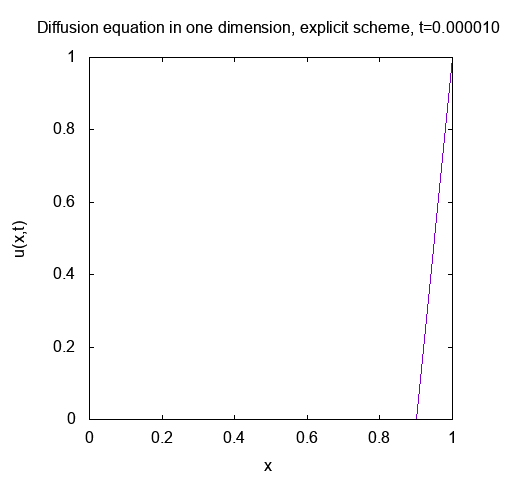
\includegraphics[scale = 0.55]{images/ex-0,1-t1.png}
                \end{minipage}
                \hspace{3cm}
                \begin{minipage}[c]{.30\linewidth}
                    \centering
                    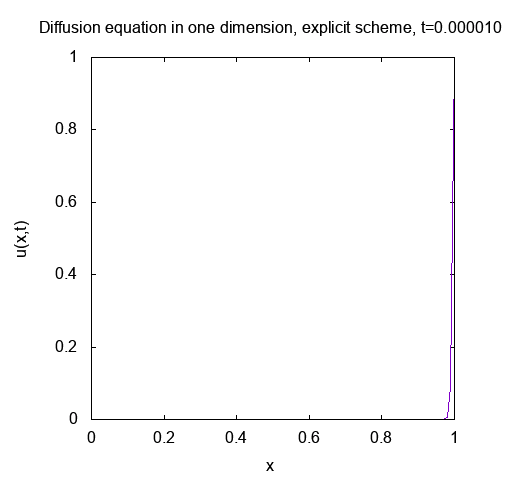
\includegraphics[scale = 0.55]{images/ex-0,01-t1.png}
                \end{minipage}
            }
            \caption{Explicit scheme for $\Delta x = \frac{1}{10}$ and $\Delta x = \frac{1}{100}$}
        \end{figure}

        \begin{figure}[h!]
            \hbox{
                \begin{minipage}[c]{.30\linewidth}
                    \centering
                    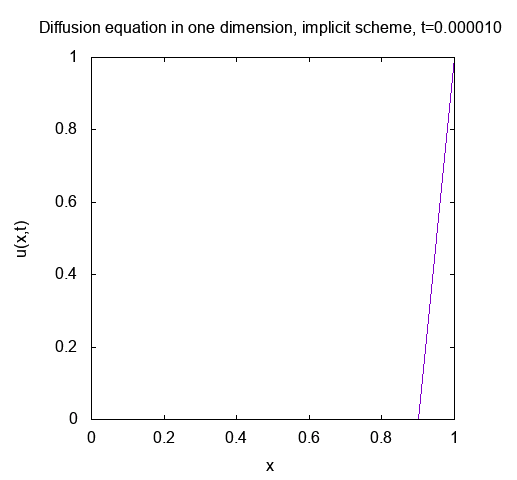
\includegraphics[scale = 0.55]{images/im-0,1-t1.png}
                \end{minipage}
                \hspace{3cm}
                \begin{minipage}[c]{.30\linewidth}
                    \centering
                    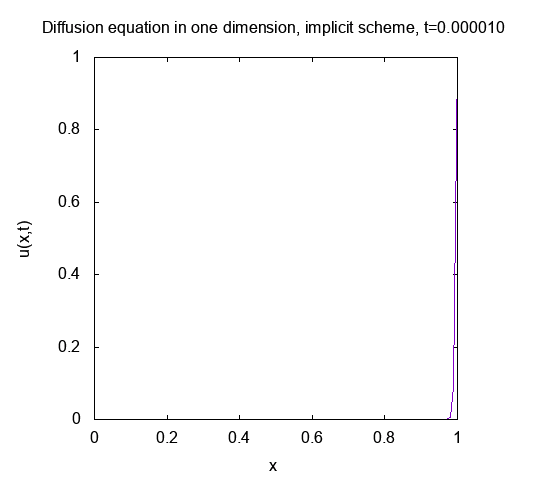
\includegraphics[scale = 0.55]{images/im-0,01-t1.png}
                \end{minipage}
            }
            \caption{Implicit scheme for $\Delta x = \frac{1}{10}$ and $\Delta x = \frac{1}{100}$}
        \end{figure}

        \begin{figure}[h!]
            \hbox{
                \begin{minipage}[c]{.30\linewidth}
                    \centering
                    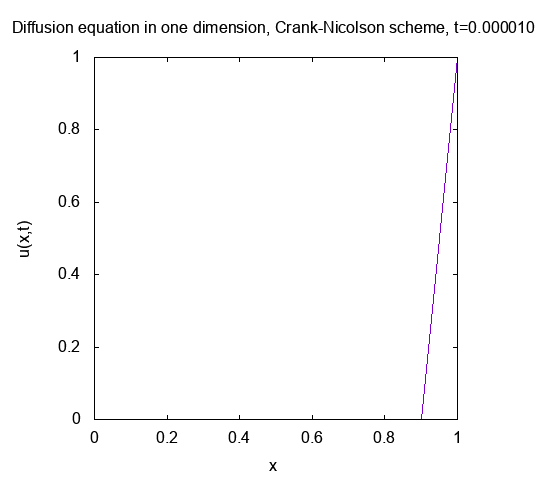
\includegraphics[scale = 0.55]{images/cn-0,1-t1.png}
                \end{minipage}
                \hspace{3cm}
                \begin{minipage}[c]{.30\linewidth}
                    \centering
                    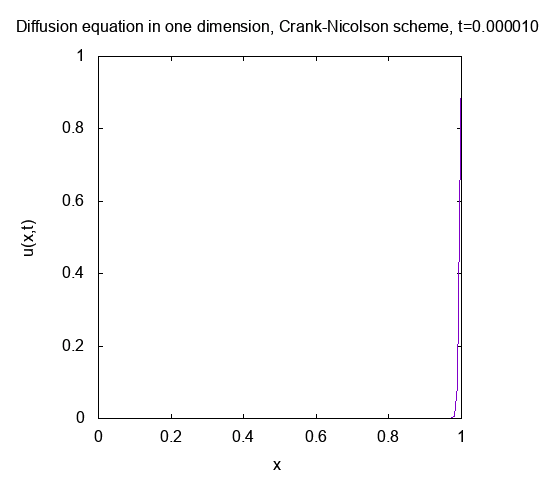
\includegraphics[scale = 0.55]{images/cn-0,01-t1.png}
                \end{minipage}
            }
               \caption{Crank-Nicolson scheme for $\Delta x = \frac{1}{10}$ and $\Delta x = \frac{1}{100}$}
            \end{figure}

            \paragraph{}As you can observe it, choosing a low precision like $\Delta x = \frac{1}{10}$ can be very dangerous for the results, even if the requirements on $\alpha$ are fulfiled. That being said, it is not clear at this time which scheme is the best.

            \newpage
            \subsection{For a time $t=0.2$}

            \begin{figure}[h!]
                \hbox{
                    \begin{minipage}[c]{.30\linewidth}
                        \centering
                        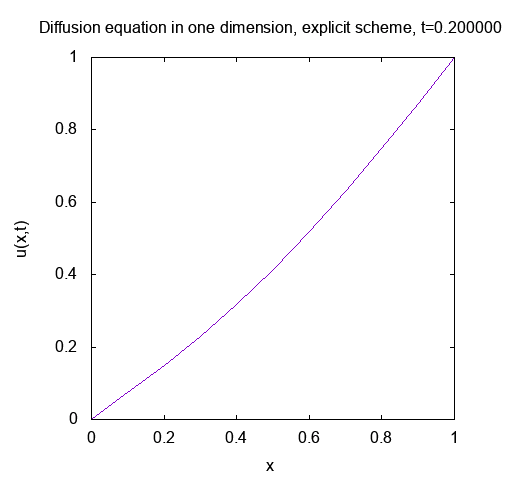
\includegraphics[scale = 0.55]{images/ex-0,1-t2.png}
                    \end{minipage}
                    \hspace{3cm}
                    \begin{minipage}[c]{.30\linewidth}
                        \centering
                        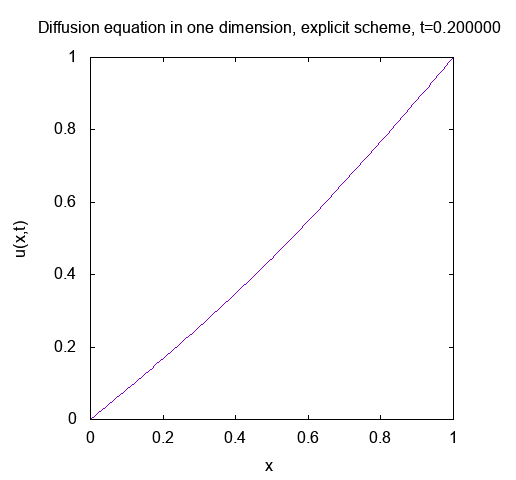
\includegraphics[scale = 0.55]{images/ex-0,01-t2.png}
                    \end{minipage}
                }
                \caption{Explicit scheme for $\Delta x = \frac{1}{10}$ and $\Delta x = \frac{1}{100}$}
            \end{figure}

            \begin{figure}[h!]
                \hbox{
                    \begin{minipage}[c]{.30\linewidth}
                        \centering
                        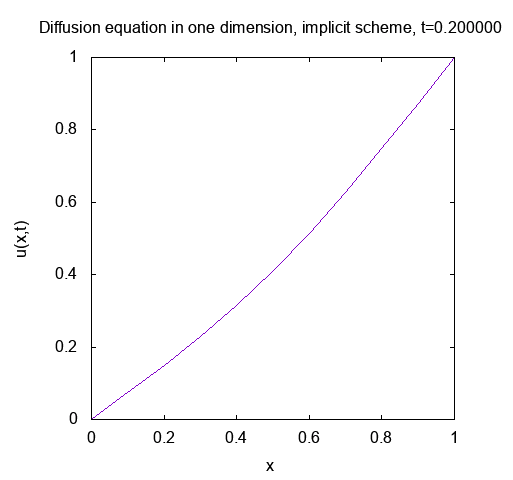
\includegraphics[scale = 0.55]{images/im-0,1-t2.png}
                    \end{minipage}
                    \hspace{3cm}
                    \begin{minipage}[c]{.30\linewidth}
                        \centering
                        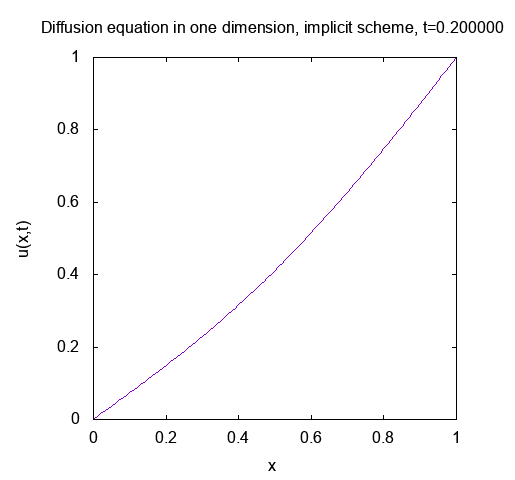
\includegraphics[scale = 0.55]{images/im-0,01-t2.png}
                    \end{minipage}
                }
                \caption{Implicit scheme for $\Delta x = \frac{1}{10}$ and $\Delta x = \frac{1}{100}$}
            \end{figure}
\newpage
            \begin{figure}[h!]
                \hbox{
                    \begin{minipage}[c]{.30\linewidth}
                        \centering
                        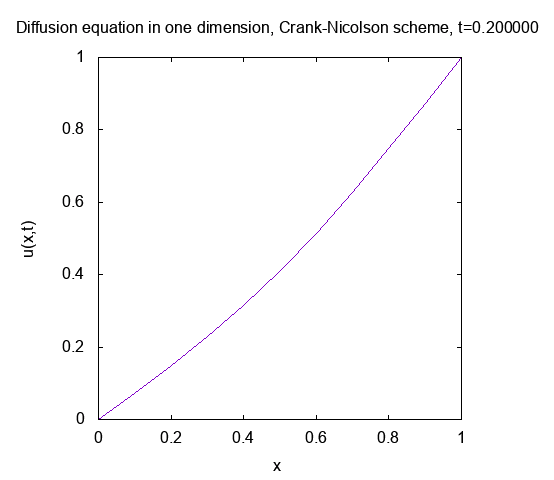
\includegraphics[scale = 0.55]{images/cn-0,1-t2.png}
                    \end{minipage}
                    \hspace{3cm}
                    \begin{minipage}[c]{.30\linewidth}
                        \centering
                        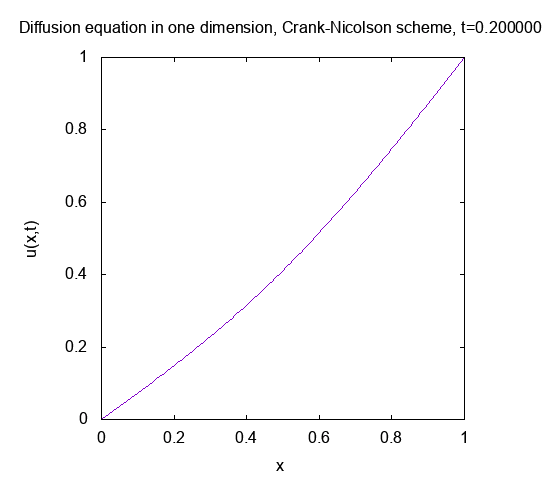
\includegraphics[scale = 0.55]{images/cn-0,01-t2.png}
                    \end{minipage}
                }
                \caption{Crank-Nicolson scheme for $\Delta x = \frac{1}{10}$ and $\Delta x = \frac{1}{100}$}
            \end{figure}

                \paragraph{}When the space-steps are increased, the differences between the schemes are not obvious and they all seem efficient. Eventually when we choose $\Delta x = \frac{1}{100}$ the curve is smoother and does not look like a set of straight lines.

            \subsection{Comparison}

                \paragraph{}On this picture it is clear that the explicit scheme is way less efficient than the others. We computed the simulations with 200 space-steps, 20000 time-steps and a final time $t=0.2$, that is we had $\alpha = 0.4$, which fulfills the stability requirements for the explicit scheme. Both the implicit scheme and the Crank-Nicolson scheme are cofounded with the analytical solution\footnote{It was plotted using the first 228 terms of the Fourier-Series and 5000 space-steps.} and they would clearly be the best choice.

                \begin{figure}[h!]
                    \begin{center}
                        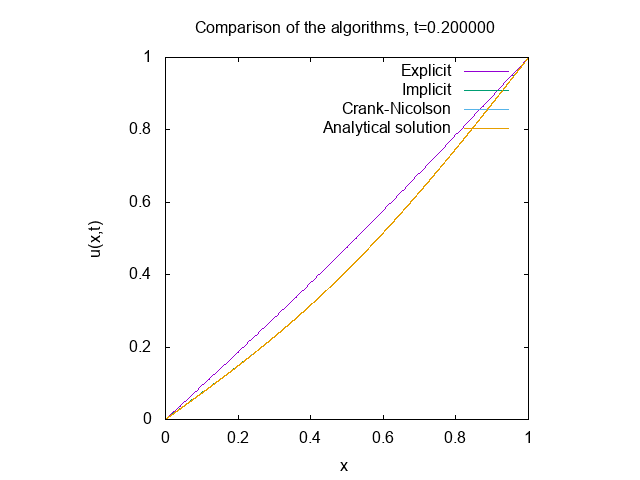
\includegraphics[width=8.5cm,height=5.5cm]{images/comparison.png}
                        \caption{Comparison of the three schemes for the same values of $\Delta x$ and $\Delta t$.}
                    \end{center}
                \end{figure}

                Even for $\Delta x = \frac{1}{100}$ they are very similar. Here are some benchmarks for those one-dimension solvers with 500 space-points, 100000 time-points and a final time $t=0.2$, which is a precision way more than sufficient. The explicit scheme is without any doubt the fastest, the Crank-Nicolson scheme is roughly 5.7 times slower, but the precision is way more accurate. Once again, it is a question of priority between speed and precision, but we would advice to choose the implicit scheme even if it is on the paper less efficient than the Crank-Nicolson scheme.

                \begin{center}
                    \begin{tabular}{|*{3}{c|}}
                        \hline
                            Explicit scheme & Implicit scheme & Crank-Nicolson scheme\\
                        \hline
                            0.1424s & 0.767s & 0.8231s \\
                        \hline
                    \end{tabular}
                    \captionof{table}{Operation times in average for the three schemes in one dimension with the above parameters.}
                \end{center}

                \paragraph{}The latter Von Neumann stability analysis will prove us that both the Implicit and the Crank-Nicolson scheme have a precision of the order ${10}^{-3}$ if we compare them with the exact solution.

        \section{Two dimensions and discussion on the diffusion process}

            \paragraph{}The two-dimensions solvers and the free boundary conditions allow to understand how diffusion of a process occur. We made short videos with this program and some bash. They show the diffusion process in time in one-dimension and two-dimensions with various boundary conditions. They are available here : \url{https://www.youtube.com/playlist?list=PL9Bkzl2Vcy4sJMAbtl1KsfRhMv7KhHTp6}.

            \paragraph{}In both one-dimension and two-dimensions we observe that the heating process is very fast at the beggining and the convergence is very slow after $t=0.001$. This convergence is a uniform convergence to a stable function which represent the steady state. We explain the slowness of the convergence by the fact that the closed form solution contains a temperature term ${e}^{-{{\lambda}_{n}}^{2}t}$ which goes to $0$ as $t$ goes to infinity, resulting in a slow convergence. Furthermore, the maximum principle for partial differential equations is verifies here because the minimum value for $u(x,y,t)$ is always the minimum of the boundary and the maximum value for $u(x,y,t)$ is always the maximum of the boundary. However the convergence occurs way before for $t<1$ for all the tested boundary conditions. The fastest convergence occurs in the \emph{Simulation 1}, and the other take longer time as they have different boundary conditions. When we apply only one heating process on one side on the lattice (\emph{Simulation 4}) instead of applying the same heating process on every side of the lattice (\emph{Simulation 1}), the convergence is also much slower.

\chapter{Stability properties of those algorithms}

    \section{Theory}

        \paragraph{}Some linear algebra tricks (again) allow us to evaluate the stability of the schemes we built. Those mathematical considerations are presented in the lecture notes, in \emph{Introduction to partial differential equations} by Tveito and Winther and in lectures by T. Lakoba from the University of Vermont. We present thereafter their results :

            \begin{center}
            \begin{tabular}{|*{3}{c|}}
                \hline
                Scheme & Truncation Error & Stability requirements\\
                \hline
                \hline
                Cranck-Nicolson & $\mathcal{O}(\Delta x^2)$ and $\mathcal{O}(\Delta t^2)$ & Stable for all $\Delta t$ and $\Delta x$ \\
                \hline
                Backward Euler & $\mathcal{O}(\Delta x^2)$ and $\mathcal{O}(\Delta t)$ & Stable for all $\Delta t$ and $\Delta x$ \\
                \hline
                Forward Euler & $\mathcal{O}(\Delta x^2)$ and $\mathcal{O}(\Delta t)$ & $\Delta t \leq \frac{1}{2}\Delta x^2$\\
                \hline
            \end{tabular}
                \captionof{table}{Comparison of the different schemes}
            \end{center}

        \paragraph{}To resume, the truncator error of the explicit scheme are laws of $\Delta x$ whereas the truncator error of the Crank-Nicolson scheme is a law of ${\Delta x}^{2}$. The best algorithm would therefore be the Crank-Nicolson scheme since it is "undoncitionnaly stable" and that it can be computed for any $\alpha$\footnote{Again it is reasonnable not to choose too few space-points.}. Intuitively we mat say that for very low times (roughly $t<0.00001$) the derivated tangent coefficient ${u}_{xx}$ undergoes jumps and irregularities since the function is hardly differentiable. An explicit scheme based on the current state and extrapolating the next step is therefore necessarely less accurate than a scheme based on more precise equations. But the Crank-Nicolson being a mix of the two paradigms is necessarely more precise.

        \paragraph{}Those mathematics can easilly be extended to a two-dimensions equation. The stability requirements for $\alpha$ are $\alpha < \frac{1}{4}$.

    \section{Observations}

        \subsection{One dimension}

            \paragraph{}The plots for the diffusion function $u$ are very convincing, and from a human eye, they all give the same results\footnote{Well maybe not for the explicit scheme.}, and those results seem very close to the analytical solution for every time $t$ as long as the value for $\alpha$ is ok. However our investigation do not match with the theory. Here is a plot of the relative error $\epsilon=\log{|\frac{{u}_{comp}(x) - {u}_{anal}(x)}{{u}_{anal}(x)}|}$ as a function of $\Delta x$. We fixed $x=0.5$, $t=0.2$ and $\Delta t = 500000$ so that we could compute the explicit scheme for many different $\Delta x$ from $\frac{1}{10}$ to $\frac{1}{1000}$.

            \begin{figure}[h!]
                \begin{center}
                    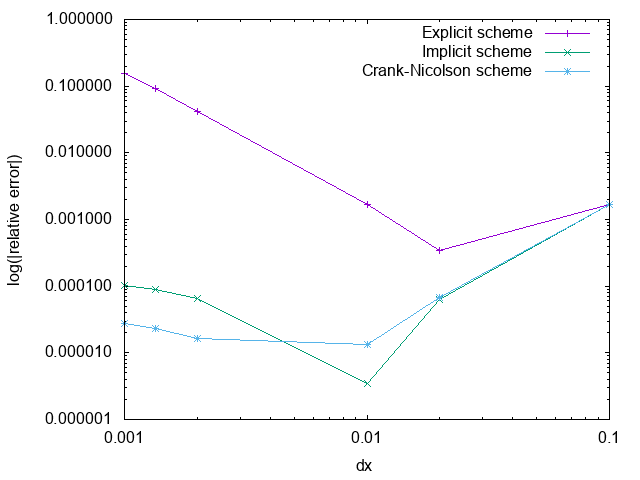
\includegraphics[scale=0.42]{images/error-dx.png}
                    \caption{Relative error of the three schemes as a function of $\Delta x$}
                \end{center}
            \end{figure}

            \paragraph{}Note also that the relative error of the Crank-Nicolson scheme does not grow as a function of ${\Delta x}^{2}$ as expected. The result is linear after a certain dx is high enough. However, the fact that in all three cases the relative error grows with \dx decreasing is mathematically irrelevant.

            \begin{figure}[h!]
                \begin{center}
                    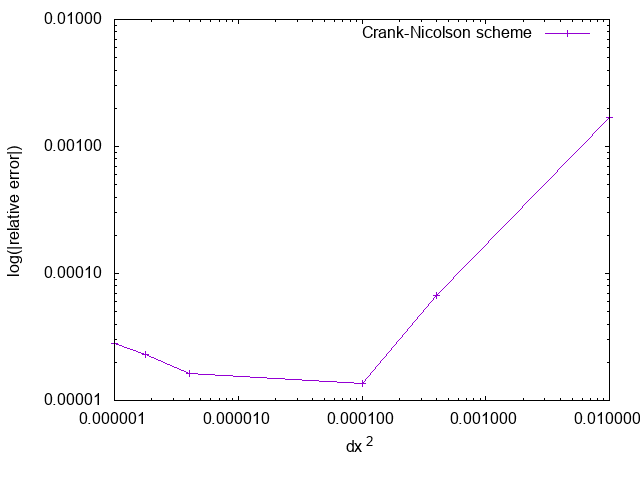
\includegraphics[scale=0.42]{images/error-dxdx.png}
                    \caption{Relative error of the Crank-Nicolson scheme as a function of ${\Delta x}^{2}$}
                \end{center}
            \end{figure}

            \paragraph{}This situation is not confortable for two reasons. Firstly this is hard to interpret because except for the explicit scheme the results of all the schemes seem relevant and reliable, secondly because this behavior is mathematically not logical and that it must be due to an implementation error. However the implementation is considered valid because the results are valid, homogeneous and reproducible, this implies that the problem is a problem of numerical precision (unlikely though) or a problem of adapting the mathematical method to an informatic concrete algorithm. In both cases this is hard to fix without spending some time investigating the code, the language and the math.

            \paragraph{}Moreover the stability of the Crank-Nicolson scheme is not "unconditional" as expected. Yet the informatic reality shows that there can be unconvenient oscillations on the curve due to the approximation of the Fourier series. The curve have the same aspect but undergoes a multiplicative factor. This can occur from times to times. Yet the error remains very acceptable for both the implicit and explicit scheme (inferior to an order of magnitude of ${10}^{-3}$) and the computation times are very fast, which lead us to consider that those solver fulfil what we expect from them, which is fast computations, reliable results and easyness to use.

        \subsection{Two dimensions}

            \paragraph{}In this part we observe that even though the alpha requirement $\alpha < \frac{1}{4}$ is fulfilled, the explicit scheme in two dimensions is not very stable and precise when $\alpha$ is greater than $0.1$. Here are some plots to prove it.
\newpage
            \begin{figure}[h!]
                \hbox{
                    \begin{minipage}[c]{.30\linewidth}
                        \centering
                        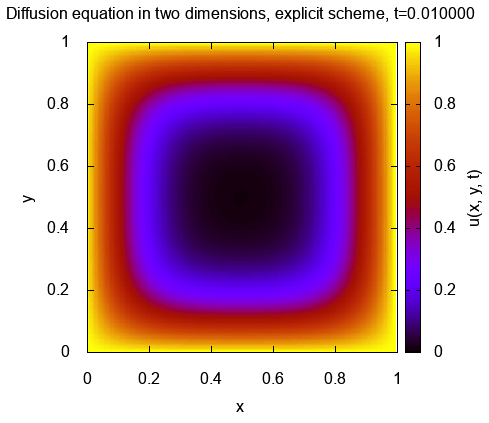
\includegraphics[scale = 0.6]{images/alpha=0,125-t1.png}
                    \end{minipage}
                    \hspace{3cm}
                    \begin{minipage}[c]{.30\linewidth}
                        \centering
                        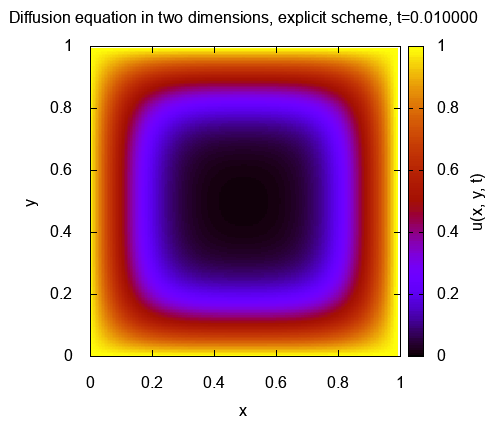
\includegraphics[scale = 0.6]{images/alpha=0,08-t1.png}
                    \end{minipage}
                }
                \caption{Implicit scheme comparison for $\alpha=0.125$ and $\alpha=0.08$}
            \end{figure}

            \paragraph{}We observe that for the biggest $\alpha$ the diffusion process looks more advanced than in the other case. This proves that the stability analysis unfortunately remains very theoritical, and can not always match the reality. The best thing to do is therefore to compare the results with other algorithms (we implemented an implicit scheme as well) and to take many precautions, such as choosing stronger requirements for $\alpha$. In our case, $\alpha < 0.1$ seems a good choice for the two-dimensions explicit solver.

            \begin{figure}[h!]
                \hbox{
                    \begin{minipage}[c]{.30\linewidth}
                        \centering
                        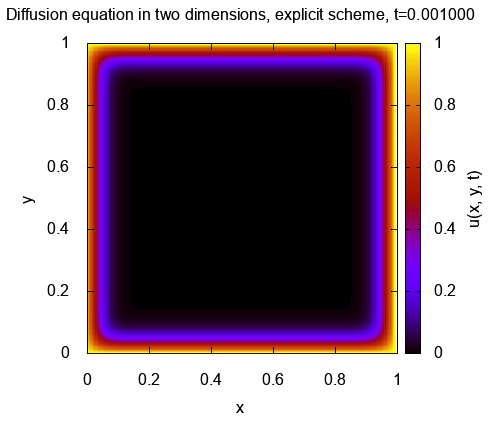
\includegraphics[scale = 0.6]{images/alpha=0,0125-t2.png}
                    \end{minipage}
                    \hspace{3cm}
                    \begin{minipage}[c]{.30\linewidth}
                        \centering
                        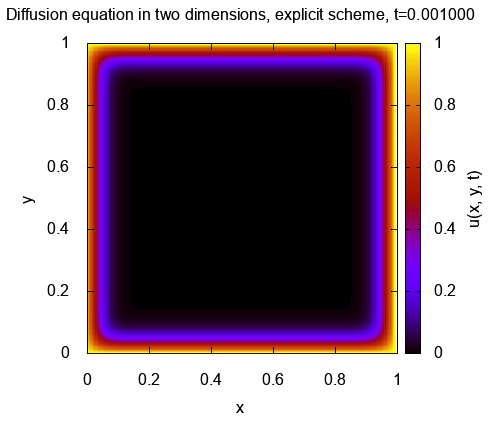
\includegraphics[scale = 0.6]{images/alpha=0,0125-t2.png}
                    \end{minipage}
                }
                \caption{Implicit scheme comparison for $\alpha=0.05$ and $\alpha=0.0125$}
            \end{figure}

            \paragraph{}This time the plots are very similar.


\chapter*{Conclusion}
\addcontentsline{toc}{chapter}{Conclusion}

    \paragraph{}The most important thing to keep in mind after this project is that stability models should not be taken for granted. The error-predictions did not match the reality even if the results were very good with wisely chosen. Since those schemes are very similar and easy to implement, it would be wise to run the implicit and the Crank-Nicolson scheme in parallel and to output the average of their results. These methods are admittedly less fast than computing the Fourier-series which is solution of the equation, but they require very basic algorithmic knowledge to be built and they can stand on previously written codes.\\
    That being said, those algorithms have the advantage of being very simple and to allow one to solve partial differential equations without requiring the mathematical background to solve those equations. After having studied those algorithms, we are know able to build larger algorithms which will need those kind of solvers.




\chapter*{Bibliography}

    \begin{itemize}

        \item{Introduction to Partial Differential Equations : A computational Approach - Aslak Tveito \& Ragnar Winther}
        \item{The Heat equation in 2 and 3 spatial dimensions - T. Lakoba}

    \end{itemize}


\end{document}
